\documentclass[10pt]{article}
\usepackage[utf8]{inputenc}
\usepackage[margin=0.5in]{geometry}

\usepackage[pdftex]{graphicx}
\usepackage{minted}
\usepackage{hyperref}
\hypersetup{
    colorlinks=true,
    linkcolor=blue,
    filecolor=magenta,      
    urlcolor=cyan,
}

\title{CS181 Practical 3: Preferences in Streaming Music}
\author{Team We Acquired WhetLab™: Victor Domene, Henrique Vaz, Joshua Meier }
\date{April 8, 2016}

\usepackage[pdftex]{graphicx}

\begin{document}

\maketitle

 It is important to note that there are about $233,000$ users and $2,000$ artists in the dataset, so the matrix representation of our data was very sparse. 


\section{Abstract}
In this practical, we performed machine learning on truncated lists of user / artist play counts, in order to predict how many times each of these users listened to every artist in the collection. The implications of high accuracy here are quite interesting - there are many commercial applications to being able to predict a user's entire play history from just a few sample points. However, this also makes the problem extremely difficult. Unlike previously practicals where we had complete training data to work with, we did not necessarily have complete data for each user in the training set, and furthermore, we had no way of even knowing {\t how} complete the data was for any user! After performing a thorough data analysis to better understand the complexity of the data, we then continued to apply a variety of very different machine learning techniques, since many different intuitions could be applied here. We also performed feature engineering, but we were unable to incorporate these features (known as "side information" in the literature) into the algorithms in a reasonable timeframe. Ultimately, we discovered that a simple matrix factorization using just a single feature performed best. Notably, our hand-crafted matrix factorization algorithm outcompeted several of the popular implementations. 

\section{Technical Approach}
\subsection{Dependencies}

We made use of a number of technologies in implementing this practical. We used Python data analysis libraries including Pandas, IPython Notebook, Numpy, Scikit-learn, and Nimfa which was installed through the Python distribution Anaconda. Additionally, we used R for data analysis and plot generation.

\subsection{Data \& Validation}
Although we were provided with a large amount of sample data in this practical (4.1M user/artist pairs in train data, 4.2M user/artist pairs in test data), we were unable to perform any cross validation due to the incomplete nature of the train data. To control for overfitting, we centered the data before performing any learning (described below).

\subsection{Data Analysis and Centering}
Before performing any feature engineering or machine learning, we began with a basic analysis of the data provided, which proved to be an essential component of our technical approach in the long run. We first began by analyzing the the spread of the data. We summed over the number of play counts for each user in the dataset, finding that the data fit a half-normal distribution with mean of $4506.2$ and standard deviation of $6467.843$. Statistics of the data are summarized in the table below:

\begin{center}
 \begin{tabular}{c c} 
\hline
\hline
mean & $4506.2$ \\
\hline
median &  $2639$ \\
\hline
standard deviation & $6467.843$ \\
\hline
max & $453683$ \\
\hline
min & $9$ \\ 
\hline
\hline
\end{tabular}
\end{center}

Notably, there was a large discrepancy between the mean and the median, due to the presence of several users who listened to an extensive amount of music. A histogram of the data further supported our observations (Figure 1).

\begin{figure}[h]
\centering
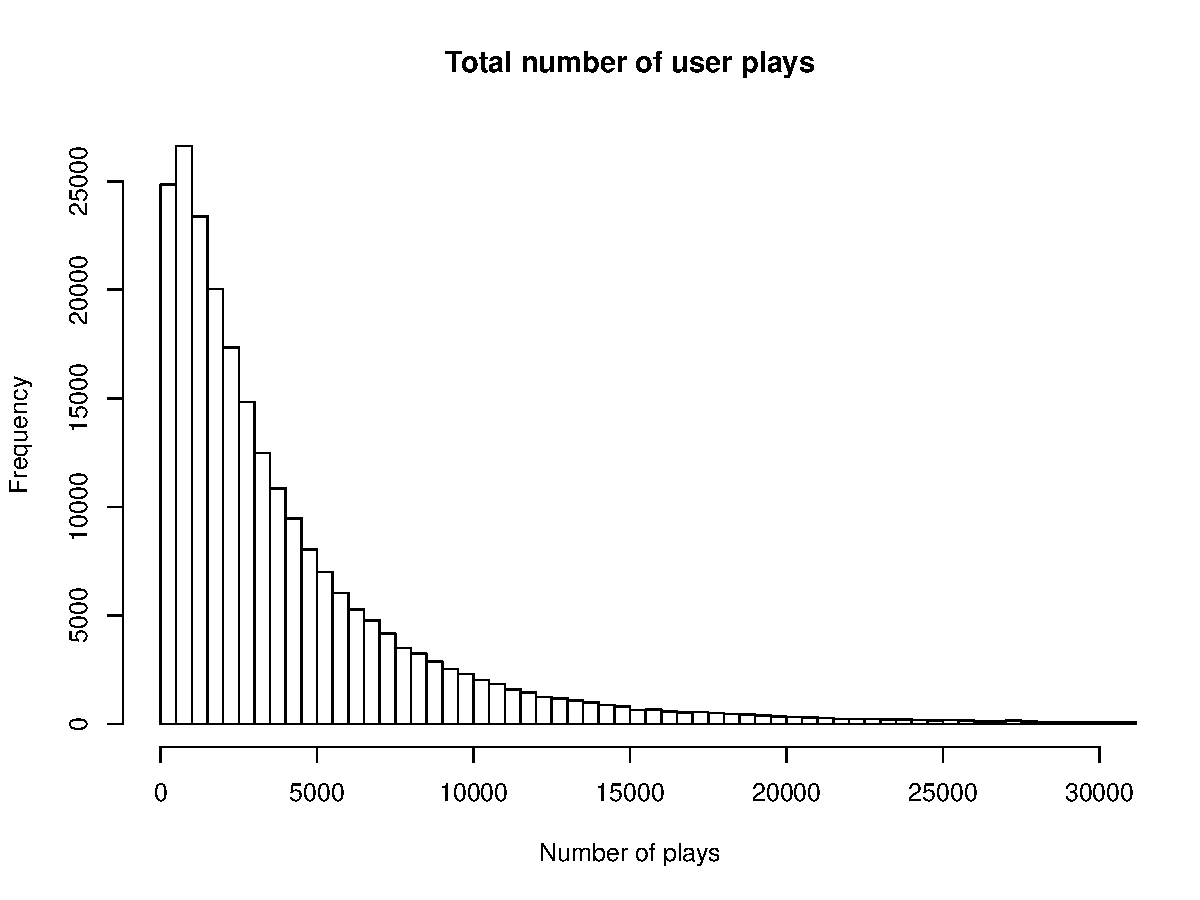
\includegraphics[width=0.8\textwidth]{../experiments/total_counts.pdf}
\caption{Histogram of the total number of user plays from the train data. This plot is right truncated since there are several users (but not many) with large number of plays. Including all this information would make it difficult to observe the half-normal distribution of the data. In particular, note that there is a user with $453683$ total plays.}
\label{fig:img3}
\end{figure}

Due to this distribution, we decided to center the data to prevent the audiophiles from biasing our results. For each user, we counted the total number of listens and divided all data for the user by this number. For validation, we plotted a histogram the data after centering (Figure 2).

\begin{figure}[h]
\centering
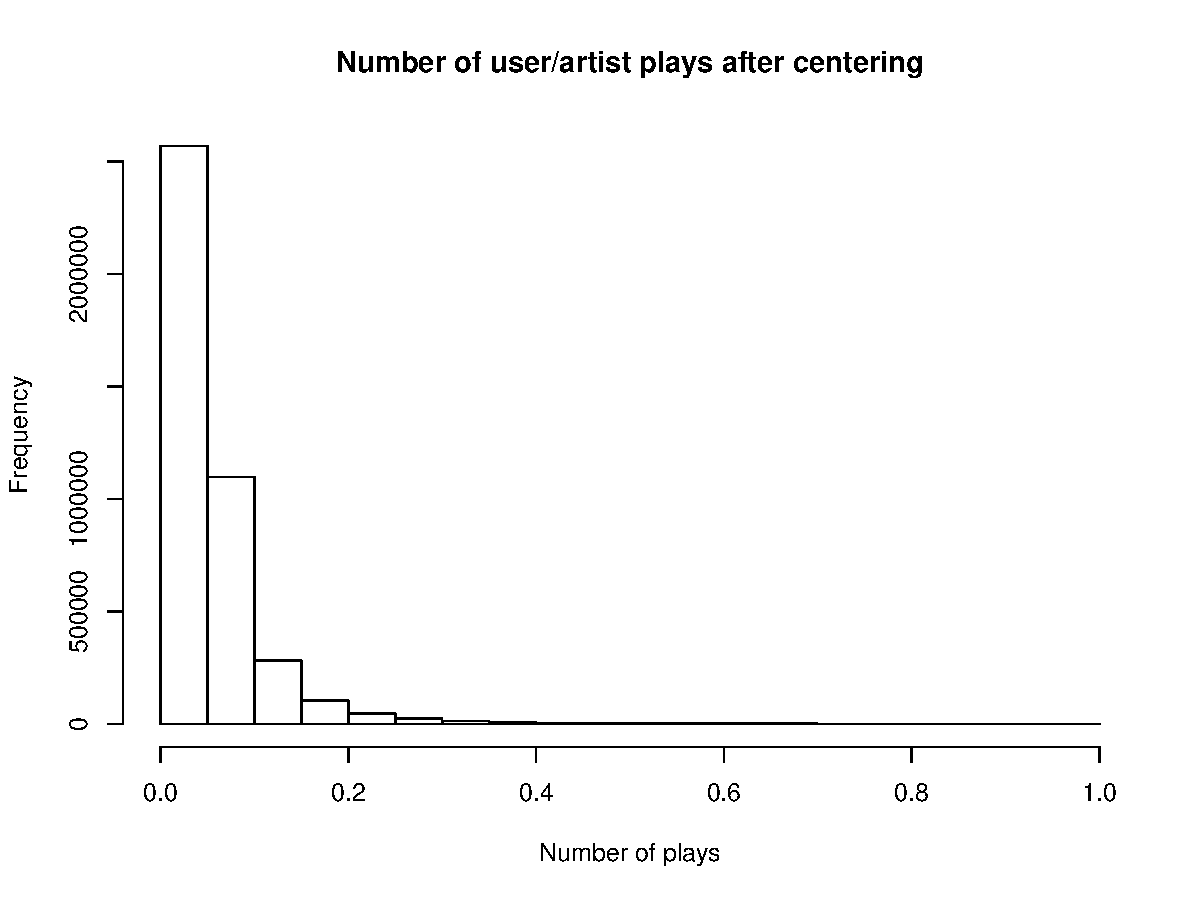
\includegraphics[width=0.8\textwidth]{../experiments/centered_train_hist.pdf}
\caption{Histogram of the total number of user plays from the train data, after centering.}
\label{fig:img3}
\end{figure}

We used the centered data in our algorithms, but we recorded the total play counts for each user so that we could un-normalize at the end. After running the machine learning, we multiplied the results by the total listen count for each user. Our intuition was to think of the algorithms as learning a probability distribution of how the user listens to each artist. We could then multiply each individual result by the total listen count. Under this intuition, the per-user median benchmark assigns identical probability to each artist. Mathematically, the probability mass function can then be expressed as
$$p(X = k) = \frac{1}{K}$$
where $K$ is the number of artists in the dataset ($2000$ here).  

\subsection{Incomplete Data}
As described above, one of the challenging properties of this practical is that the training data is incomplete. Initially, we assumed that we could just focus our learning algorithms on the data that was more "complete." However, a closer analysis of the data realized that the data was evenly spread out, making it difficult to put a metric on how "complete" the data is. (Even though we might have a lot of data on a user, it is still possible that much more is missing.) We plotted a histogram of the artists count per user (Figure 3).

\begin{figure}[h]
\centering
\includegraphics[width=0.8\textwidth]{../experiments/count_artists_histogram.png}
\caption{Number of artists each user has listened to, in the train data.}
\label{fig:img3}
\end{figure}

\subsection{Demographic Information}
We intuitively believed that demographic information (as provided in profiles.csv) would be very valuable for this practical, as it allows us to group various sets of users together. Surprisingly, we were not able to find much literature or open-source code on incorporating demographic information into the Netflix Challenge (or other similar variants), although when we changed our search term to "Side Information," we picked up various interesting papers.

However, upon reading the demographic information in more depth, we discovered several notable discrepancies. In particular, we have data on people from North Korea and data on people who are negative age. This is highly suspicious, but we decided to incorporate this information anyway, due to the lack of a systematic technique to clean the data.

\subsection{Feature Engineering}
We next conducted some basic feature engineering, although as described above, we had difficulty using it in some of our algorithms. We first started with the musicbrainz-python API, but we could only download around $3$ entires per second, which is too slow for the massive dataset we have. Instead, we set up a local server using the musicbrainz data (database size: 2GB), to speed up the computation. We extracted the tags in the tag-list portion of the XML describing each artist, which represent the genres of each artist. This allowed us to narrow the data from $2000$ classes to just a few for some analyses.

\subsection{Algorithms}
We tested a wide variety of learning algorithms for this practical. We could not use cross-validation due to the nature of this practical, so all results are reported as the scores provided by Kaggle. However, we did compute reconstruction errors for the training data for some of the methods (in particular, for those that seemed to work best).

\subsubsection{Per-user Median}
We submitted the per-user median, according to the sample code provided by staff. The Kaggle score was $137.79$. This approach yielded a $129.54$ reconstruction error.

\subsubsection{Global Median}
We submitted the global median, according to the sample code provided by staff. The Kaggle score was ----.

\subsubsection{Random Forests}
Here, we considered the practical as $2000$ supervised learning problems, where the goal is to predict a single artist from the data provided about each user. In a pre-processing step, we formed a matrix of  play counts between users and artists, filling in $0$s when there is no indication that a user listened to an artist. (We were not thrilled with this approach, since we do not really know whether those values should really be $0$, and that could influence our results. However, we thought this approach might perform better than the benchmark). We then trained $2000$ random forests where the training data is the play counts for each artist (besides the one we are predicting) and the goal is to predict that artist. Of course, for users where we know the result for that artist, we might get a different value with the random forest. Therefore, in a post-processing step, we super-impose the training matrix on top of the result matrix, only using the values from the result matrix if the training matrix has a $0$ in that cell. We then go through the testing data user / artist pairs and read the values off of the final results matrix.

As expected, this approach took a long time to run. We therefore rented an AWS node with 64GB of memory (necessary since the matrices are so sparse), and ran this experiment there. It took around 10-15 hours to fit the random forests. During the prediction stage, we periodically analyzed the results that were being predicted using the Unix {\it less} reader. We discovered that the results printed were very low (less than $1$ in most cases), so we decided to abandon this approach. We hypothesize that the large number of $0$s in the matrix biased the results in that direction. We never submitted these results to Kaggle because they were clearly very poor and we did not want to waste one of our limited entries.

\subsubsection{Matrix Factorization}
It is obvious from the literature that matrix factorization techniques are popular for rating prediction tasks. For example, there are many technical blog posts from Spotify and Netflix describing their machine learning approaches to determine how a user would rate new music or movies. These services then suggest that the user engage with content that they are likely to rate highly. Additionally, course staff provided $3$ valuable references on matrix factorization, which we tried implementing (a) from scikit-learn; (b) from Nimfa; and (c) manually.

{\bf Scikit-learn Matrix Factorization:}

In particular, we used the class called sklearn.decomposition.NMF. Surprisingly, this library only seems to provide the basis vectors for the matrix factorization and does not expose the weights. In order to make practical use of this library, we need access to those weights. We were not alone in this assumption - we approached Finale about this issue, and several students commented about it on Piazza. This seems to be a flaw in the Scikit-learn library and we therefore submitted a Bug Report through the Issues page on the Scikit-learn GitHub.

{\bf Nimfa Matrix Factorization:}

This library works similar to the scikit-learn one, however it exposes the information we require! It also has many tunable parameters. When assuming low matrix rank, the algorithm terminates in reasonable time, but we achieve a bad Kaggle score around ----.  In fact, Nimfa has a method for automatically determining the proper rank, but we did not make use of that method because it takes a long time. (Essentially, it tries the algorithm on many possible ranks and looks at whatever gives the best objective function.) On high rank though, the algorithm takes an unreasonable amount of time - we terminated our run of rank$=30$ (the default) after the algorithm did not terminate when running overnight. The internal workings here are very abstracted from us, we sought to code our own matrix factorization.

{\bf Manual Matrix Factorization:}
After working on the methods described above, we started to think that the data has not much information to be truly learned. As a consequence, we thought that the simplest possible model would be able to give us better results. We then came up with the following idea. Each user has a "user frequency", while each artist has a "popularity". The number of predicted plays is simply the product of these two. To optimize, we used stochastic gradient descent, as specified in the \href{https://datajobs.com/data-science-repo/Recommender-Systems-[Netflix].pdf}{Vollinsky paper}. In particular, we followed the Alternating Least Squares approach. In the end, this method is simply a matrix factorization for a single feature (namely, rank$=1$ in Nimfa), but since we were not sure about the approach that these given libraries used, we hoped that by manually facturing our factorization we would get some improvements.

To be able to evaluate how good the model is, we calculated the reconstruction error for our predictions. We tried several implementations. First, we tried centering the data around the median. This gave us a reconstruction error of $144.97$. Then, we tried instead of centering, adding a bias term to the predictions and objective function; this resulted in a reconstruction error of $142.31$. Then, we decided to not use biases or centering, but instead to initialize the factorization matrices in a clever way: for each user, the frequency is its median, and for each artist, its popularity is $1$. This naive approach proved the most successful.

For $20$ iterations of our method, the reconstruction error was $128.16$. After $30$ iterations, the reconstruction error was $127.98$. The corresponding Kaggle score was $136.30$, which gave us the fourth position in the Public Leaderboard (as of 2pm on Friday). 

\section{Code}

The code for this practical can be found in this \href{https://github.com/victordomene/cs181-practicals/tree/master/practical3}{GitHub Repository}. There is a README file with some setup instructions.

\end{document}
